\input{../preamble.tex}

\graphicspath{ {../images/} }

\begin{document}
    
% Indicate your name and your student number here (e.g., A01xxx)
\header{Lab 2}{Wira Azmoon Ahmad}{A0149286R}

%======================================
\section{Learning Rate}

The first step was to increase the learning rate from 0.001 to 0.01.
As given in the hint, this improved the performance greatly, 
to around $60\%$.

\section{Pretrained Model}

Using the provided AlexNet \cite{alex12} pretrained model 
in PyTorch \cite{torch},
performance can be further improved.
Since much research has already been done on developing 
convolutional neural networks (CNN) to classify images,
it is not prudent to reinvent the wheel for this task.
AlexNet was chosen since its performance fit very well,
achieving high training validation of around $80\%$ on the dataset.
Furthermore, it is relatively simple to implement for the task
as seen in the short lines of code in \texttt{Model.py}.
The model can be trained within 10 epochs.
It is possible to continue traininig until 
train accuracy is very close to $100\%$,
but this did not further improve validation accuracy.
The chosen hyperparameters using Stochastic Gradient Descent (SGD)
were the learning rate $\alpha=0.001$ and 
weight decay $\lambda=0.01$.
Empirically, changing these values did not improve performance.

\newpage
\section{AlexNet}

AlexNet's architecture consists of five convolutional layers,
and three fully-connected (FC) layers, as seen in the diagram below.
The CNN layers were left untouched, while the FC layers were
slightly modified to include the intention as \texttt{in\_features}
for the first FC layer
and the \texttt{out\_features = num\_bins} from the last FC layer.
The architecture also included dropout on some activations,
as a regularization effect.

\begin{figure}[h]
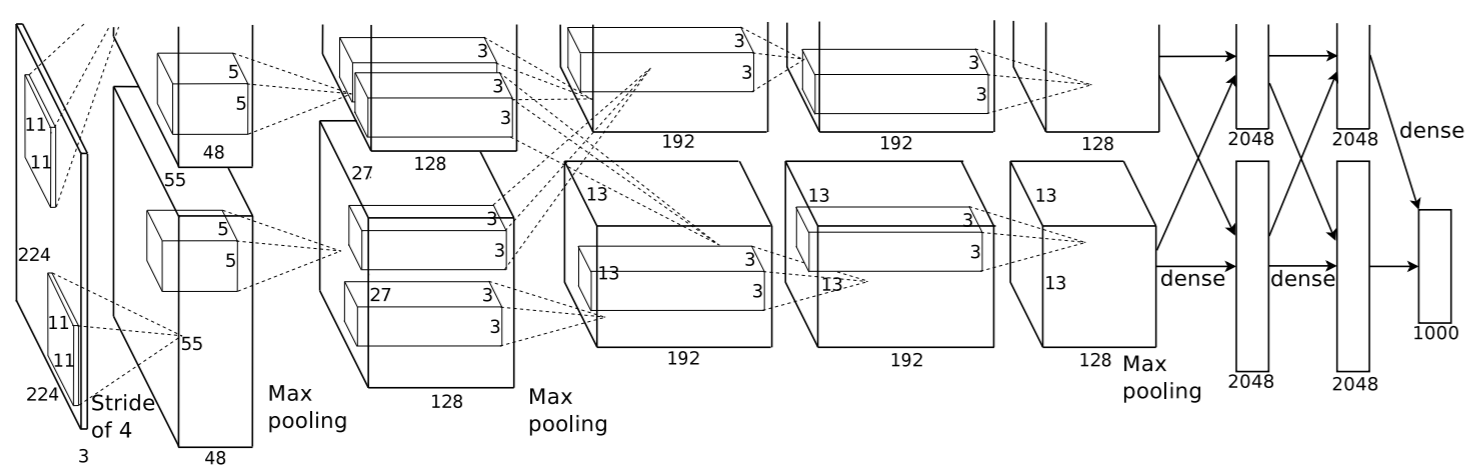
\includegraphics[width=\textwidth]{alexnet.png}
\caption{Architecture of AlexNet}
\end{figure}

\section{Dataset}

AlexNet was trained on ImageNet \cite{ILSVRC15}, 
a dataset of over 15 million labeled 
high-resolution images, categorized to around 22,000 categories.

\newpage
\section{Data Augmentation}

The data had a 0.5 probability of flipping horizontally,
with the appropriate change in the user intention and velocity label.
Some data augmentation was attempted, including random
\begin{enumerate}
    \item Rotation
    \item Cropping
    \item Blurring
    \item Perspective
    \item AutoContrast
\end{enumerate}
This only improved performance very marginally, by around $1\%$.

\section{Other}

Other attempts for finetuning were made but failed to improve performance.
\begin{enumerate}
    \item Using Adam optimizer
    \item Using GoogLeNet / Inception as the models
\end{enumerate}

\newpage
\bibliographystyle{abbrv}
\bibliography{../ref}

\end{document}